\chapter{Les cycles thermodynamiques}
\section{Introduction}
Un \textbf{cycle} est un ensemble de transformation après lesquelles 
le fluide moteur retourne à son état initial. Un cycle est dit 
\textbf{idéal} lorsqu'il approxime un processus réel. Il s'agit d'une 
approche pratique simplifiée mais non exacte. Dans la réalité, il y a 
toujours des pertes de charges (cf. \textit{PDT}),\dots

	\subsection{Travail réversible}
	Le travail des cycles moteurs est différent si le système est 
	ouvert ou fermé :
	\begin{itemize}
	\item[$\bullet$] Systèmes fermés 
	\begin{equation}
	dw_{rev} = -p.dv
	\end{equation}
	\item[$\bullet$] Systèmes ouverts
	\begin{equation}
	dw_{rev} = v.dp
	\end{equation}
	\end{itemize}
	Il existe toute une série d'expression du travail associés à différents 
	systèmes en fonction des propriétés, liste non reprise ici.
	
	\subsection{Diagramme entropique}
	Il s'agit d'un diagramme $(T,s)$, utilisé pour les échanges de chaleurs 
	car l'aire sous une transformation réversible est la quantité de chaleur 
	échangée 
	\begin{equation}
	\delta q_{rev} = T.ds
	\end{equation}
	L'entropie d'un gaz parfait s'écrit 
	\begin{equation}
	ds = c_p\dfrac{dT}{T}-R\dfrac{dp}{p} = c_v\dfrac{dT}{T}+R\dfrac{dv}{v}
	\end{equation}
	Dans un tel diagramme, les transformations adiabatiques seront représenté 
	par une ligne verticale et les $p,v=\ cste$ par une fonction exponentielle :
	\begin{equation}
	\begin{array}{llll}
	p =\ cste &; ds = c_p\frac{dT}{T},& s = c_p\ln T + B, & T = ke^{\frac{s}{c_p}}\\
	v =\ cste &; ds = c_v\frac{dT}{T},& s = c_v\ln T + B, & T = ke^{\frac{s}{c_v}}	
	\end{array}
	\end{equation}
	\begin{center}
	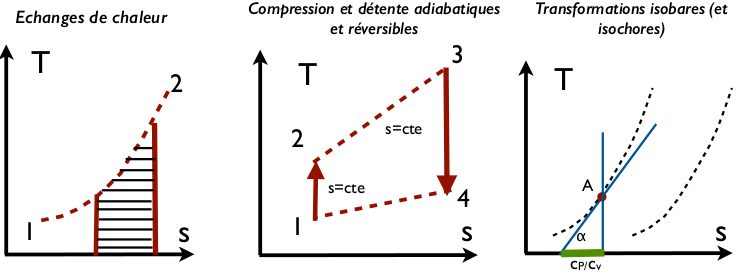
\includegraphics[scale=0.45]{ch9/image1.png}
	\captionof{figure}{NB : $T/C_p = dT/ds = \tan\alpha$}
	\end{center}	
	Dans un diagramme entropique, les isobares et isochores se déduisent par simple
	translations.
	
	\subsection{Diagramme du travail}
	Il s'agit du classique, le diagramme $(p,v)$, très pratique pour les échanges de 
	travail car l'aire située sous une transformation vaut le travail échangé. 
	\begin{equation}
	pv^n=\ cste,\qquad pv = RT\qquad \rightarrow \left\{\begin{array}{ll}
	Tp^{\frac{1-n}{n}}=\ cste\\
	Tv^{n-1}=\ cste	
	\end{array}\right.
	\end{equation}		
	Les transformations polytropiques se représentent ainsi comme des hyperboles 
	et les autres ($p,v=\ cste$) par des lignes droites.
	\begin{center}
	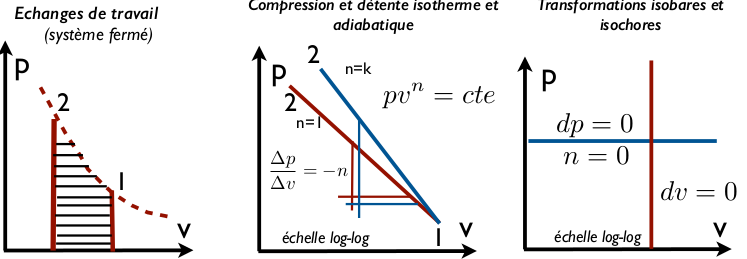
\includegraphics[scale=0.45]{ch9/image2.png}
	\captionof{figure}{Diagrammes $(p,v)$}
	\end{center}	
	
	
	
\section{Cycles à vapeur}
	\subsection{Le cycle de Rankine}		
	Il s'agit du cycle idéal des centrales thermiques à vapeur d'eau. L'idée est 
	qu'une pompe comprime de l'eau (le travail de compression doit être minimal 
	par rapport à celui de la turbine). Une fois comprimé à l'état de liquide 
	saturé, on le chauffe jusqu'à l'état de vapeur saturé pour ensuite le faire 
	détendre dans la turbine. Notre source "froide" est donnée par la condenseur.\\
	Ces quatre étapes sont les suivantes :
	\begin{description}
	\item[1-2] compression adiabatique et réversible dans la pompe (à partir de 
	l'état liquide saturé)
	\item[2-3] échange de chaleur isobare jusqu'à l'état de vapeur saturée
	\item[3-4] détente adiabatique réversible dans la turbine
	\item[4-1] échange de chaleur isobare dans le condenseur
	\end{description}
	\begin{center}
	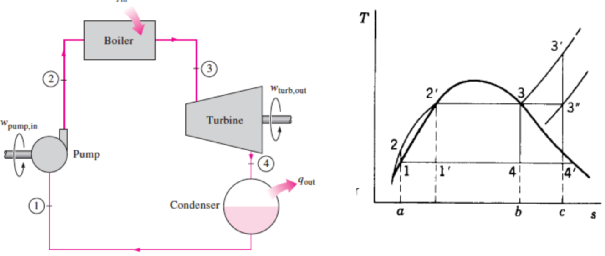
\includegraphics[scale=0.5]{ch9/image3.png}
	\captionof{figure}{Cycle de Rankine}
	\end{center}

	\danger Si on passe dans un surchauffeur, il s'agit du cycle de  Hirn et non 
	plus de Rankine ! Sur le schéma ci-dessus, 3-4 correspond au cycle de Rankine 
	et 3'-4' au cycle de Hirn.
	
		\subsubsection{Travail}
		\begin{wrapfigure}[8]{l}{4cm}
		\vspace{-5mm}
		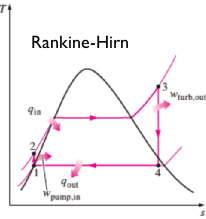
\includegraphics[scale=0.45]{ch9/image4.png}
		\captionof{figure}{ }
		\end{wrapfigure}
		Plus la différence de volume massique entre les phases de détente et de 
		compression est grande, plus le travail effectué sera grand :
		\begin{equation}
		w_{net} = w_{turbine}^* - w_{pompe}
		\end{equation}
		Pour maximiser cette différence, on effectue un changement de phase 
		\begin{equation}
		\begin{array}{ll}
		w_{pompe} &= v_L \int_{p_1}^{p_2} dp = v_L(p_2-p_1)\\
		w_{turbune} &= \int_{p_4}^{p_3} v_Vdp
		\end{array}
		\end{equation}
		Dans ces conditions, le travail de la pompe sera 1k plus petit que celui 
		de la turbine : on le néglige
		\begin{equation}
		v_L \ll v_V \rightarrow w_{pompe} \ll |w_{turbine}|
		\end{equation}
		Pour effectuer le changement de phase, on surchauffe la vapeur avant de 
		la détendre : c'est le \textbf{cycle de Hirn}
		
		\subsubsection{Analyse énergétique}
		\begin{wrapfigure}[8]{r}{4cm}
		\vspace{-5mm}
		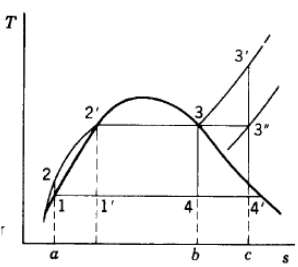
\includegraphics[scale=0.45]{ch9/image5.png}
		\captionof{figure}{ }
		\end{wrapfigure}
		On considère un système \textbf{ouvert} ($q+w = h_2-h_1$), stationnaire, 
		une entrée/sortie et pas de variation de $T$ et $V$. Faisons le bilan :
		\begin{description}
		\item[Pompe ($q=0$)] $w_{pompe} = h_2-h_1 = v(p_2-p_1)=1/\rho(p_2-p_1)$
		\item[Chaudière ($w=0$)] $q_{in} = h_3-h_2$
		\item[Turbine ($q=0)$] $w_{turbine}^* = h_3-h_4$
		\item[Condenseur $(w=0)$] $q_{out} = h_1-h_4$
		\end{description}
		L'effifacité thermique vaut dès lors 
		\begin{equation}
		\epsilon_{th} = \dfrac{\text{aire } 1-2-2'-3-4-1}{\text{aire } a-2-2'-3-b-a}
		\end{equation}
		Ou encore 
		\begin{equation}
		\epsilon_{th} = \dfrac{w_{turbine}^*-w_{pompe}}{q_{in}} = \dfrac{q_{in}-|q_{out}|}{
		q_{in}} = 1-\dfrac{|q_{out}|}{q_{in}}
		\end{equation}
		On remarque que cette expression est proche du cycle de Carnot. En fait, c'est 
		le cycle qui s'en rapproche le plus. La seule différence avec le cycle de Carnot 
		est que les deux isobares ont été remplacés par des isothermes, rendant sa 
		réalisation possible. 
		
		\newpage
		\subsubsection{Cycle idéal vs cycle réel}
		Le fait d’être le cycle de Carnot pour les centrales thermiques lui offre un 
		rendement exergétique de plus de 80\%. Cependant, il possède plusieurs 
		inconvénients :
		\begin{itemize}
		\item[$\bullet$] Mettre le condenseur sous-vide pour utiliser l'ambiance 
		comme source froide est difficile
		\item[$\bullet$] Condensation partielle dans la turbine. Si le titre de 
		vapeur est inférieur à 0.88, l’érosion débarque
		\item[$\bullet$] Pertes en tuyauterie (charge et chaleur vers l'ambiance)
		\item[$\bullet$] Pertes en turbines et dans la pompe (dissipation visqueuse)
		\item[$\bullet$] Pertes dans le condenseur (refroidissement sous la température de saturation
		\item[$\bullet$] Manque une petite image slide 21 ça serait bien
		\end{itemize}
	
	\subsection{Le cycle de Rankine-Hirn}
		\subsubsection{Améliorations possibles du cycle}
		\begin{wrapfigure}[8]{l}{3.5cm}
		\vspace{-5mm}
		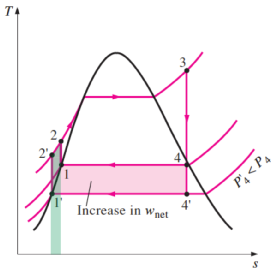
\includegraphics[scale=0.35]{ch9/image6.png}
		\captionof{figure}{ }
		\end{wrapfigure}
		On peut diminuer la pression dans le condensateur, cela augmente le 
		travail net (rose, $1'-2'-2-1-4'-4$), la chaleur fourmie au liquide 
		augmente aussi (augmente de $2'-2$, vert) et l'efficacité thermique 
		augmente aussi. Cependant, réduire la pression réduit le titre, le rendement et le 
		risque d'érosion augmente.\\\\
		\\
		
		
		\begin{wrapfigure}[8]{r}{3.cm}
		\vspace{-15mm}
		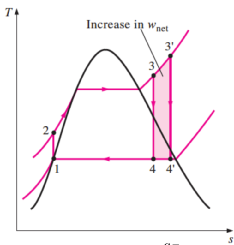
\includegraphics[scale=0.35]{ch9/image7.png}
		\captionof{figure}{ }
		\end{wrapfigure}
		Un autre moyen de faire est de surchauffer la vapeur. Le travail net 
		augmente (rose), la chaleur fournie au liquide aussi ($3-3'$), l'effet 
		net est une augmentation de l’efficacité et la teneur en eau en 4' 
		diminue. Hélas, l'irréversibilité augmente, la totalité du chauffage 
		est irréversible : le rendement exergétique diminue.\\\\
		
		
		\begin{wrapfigure}[7]{l}{3.cm}
		\vspace{-8mm}
		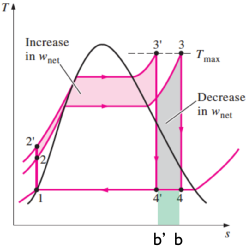
\includegraphics[scale=0.35]{ch9/image8.png}
		\captionof{figure}{ }
		\end{wrapfigure}		
		Troisième amélioration possible : augmenter la pression maximale. Le 
		travail net augmente (rose) et diminue en même temps (gris) : $w_{net}$ 
		est constant. Par contre, la chaleur rejetée par l'air diminue $4'-4-b
		-b'-4'$ et le rendement exergétique augmente. L'inconvénient est que la 
		teneur en eau augmente.\\
		\\
		
		\subsubsection{Alternative : cycle à resurchauffe}
		On introduit une ou plusieurs surfchauffe : l'efficacité est presque 
		constante, mais la teneur en eau est réduit. L'idée est de faire une 
		détente incomplète puis de la re-réchauffer et effectuer une deuxième 
		détente, cette fois-ci complète. Ca fonctionne, mais il faut deux 
		turbines!
		\begin{center}
				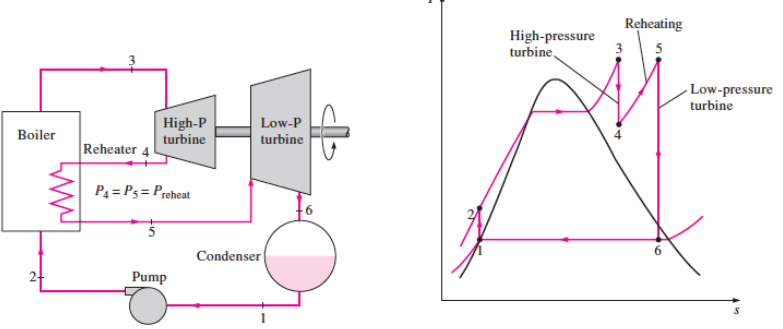
\includegraphics[scale=0.45]{ch9/image9.png}
		\captionof{figure}{Cycle à resurchauffe}
		\end{center}
	
		\subsubsection{Alternative : cycle a soutirage}
		La basse température est un problème niveau exergétique (on perd la plus 
		part de notre exergie). Ici, l'idée est de prélever une fraction de vapeur 
		dans la turbine à une pression intermédiaire pour réchauffer l'eau à la sortie 
		de la pompe. C'est mieux, car rajouter une turbine est plus compliqué 
		que de rajouter une pompe.
				\begin{center}
				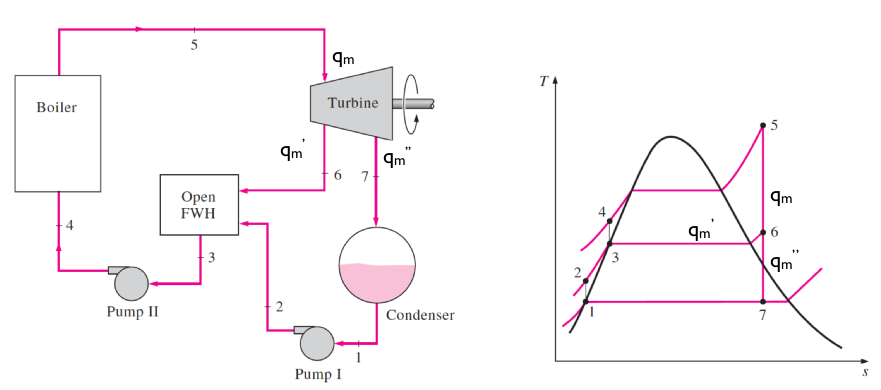
\includegraphics[scale=0.4]{ch9/image10.png}
		\captionof{figure}{Cycle à soutirage}
		\end{center}
		En pratique, plusieurs soutirages et des réchauffeurs d’eau à mélange
		sont utilisés. \textit{Le calcul du rendement est simple, mais pas intéressant.}
		
		
\newpage
\section{Cycles à gaz}
	\subsection{Intro : moteurs à combustion interne}
	Avant d'étudier ces moteurs, il est nécessaire de formuler quelques hypothèses: le 
	débit d'air est constant, le gaz est comme moi PARFAIT (au cas ou) ($c_p$), la combustion est remplacée 
	par un échangeur de chaleur d'une source externe. De plus, on complète le cycle par 
	un échange de chaleur avec l'ambiance (remplace l'admission/échappement) et toutes 
	les transformations sont supposées réversibles.
	
	\subsection{Cycle de Joule-Brayton}
		\subsubsection{Cycle idéal}
		\begin{wrapfigure}[11]{l}{10cm}
		\vspace{-5mm}
	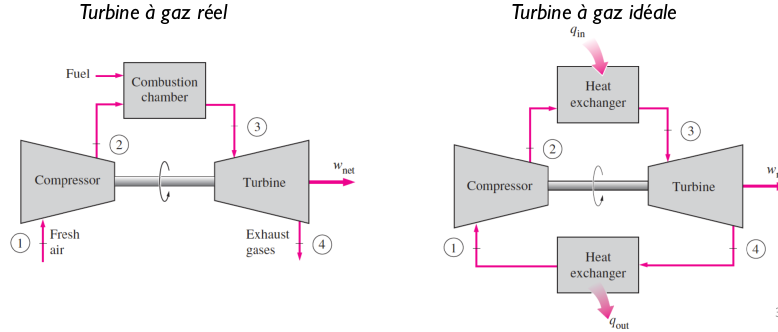
\includegraphics[scale=0.35]{ch9/image11.png}
	\captionof{figure}{Cycle de Joule-Brayton}
		\end{wrapfigure}			
	Il s'agit du cycle \textbf{idéal} pour les turbines à gaz, composé de deux échanges 
	de chaleurs isobares et deux variations de pressions isentropiques, exactement comme 
	le cycle de Rankine à une exception : le fluide est \textbf{toujours} à l'état 
	gazeux.\\
	
	Procédons à l'analyse énergétique. Nous savons que les échanges de chaleurs sont 
	isobares ($q = \Delta h$) et que la compression/détente sont adiabatiques ($w=\Delta h$).
	
	\begin{itemize}
	\item[$\bullet$] Compresseur ($q=0$) : $w_c = h_2-h_1 = c_p(T_2-T_1)$
	\item[$\bullet$] Chambre de combustion ($w=0$) : $q_{in} = h_3-h_2 = c_p(T_3-T_2)$
	\item[$\bullet$] Turbine ($q=0$) : $w^*_t = h_3-h_4 = c_p(T_3-T_4)$
	\item[$\bullet$] Échangeur ($w=0$) : $q_{out} = h_1-h_4 = c_p(T_1-T_4)$
	\end{itemize}
	L'efficacité thermique se définit alors (\textbf{attention} au $-w_p$ !) :
	\begin{equation}
	\epsilon_{th} = \dfrac{w_t^*-w_p}{q_{in}} = \dfrac{q_{in}-|q_{out}|}{q_{in}} = 1-
	\dfrac{|q_{out}|}{q_{in}}
	\end{equation}
	Avec nos expressions fraîchement écrites, on trouve
	\begin{equation}
	\epsilon_{th} = 1-\dfrac{T_4-T_1}{T_3-T_2} - 1-\dfrac{T_1(T_4/T_1-1)}{T_2(T_3/T_2-1)}
	\end{equation}
	Il est possible de ré-écrire ce rendement en fonction du taux du compression $\Pi$ en 
	utilisant les transformations adiabatiques réversibles ($pv^k =\ cste$) :
	\begin{equation}
	T_2 = T_1 \dfrac{P_2^{\frac{k-1}{k}}}{P_1} = T_1\Pi^{\frac{k-1}{k}}, \quad 
	T_3 = T_4 \dfrac{P_2^{\frac{k-1}{k}}}{P_1} = T_4\Pi^{\frac{k-1}{k}}, \quad k = \dfrac{c_p}{
	c_v}.
	\end{equation}
	On en déduit que
	\begin{equation}
	\dfrac{T_4}{T_1}=\dfrac{T_3}{T_2},n \qquad \dfrac{T_1}{T_2} = \dfrac{1}{\Pi^{\frac{k-1}{k}}}
	\end{equation}
	Le rendement s'écrit alors 
	\begin{equation}
	\epsilon_{th} = 1- \dfrac{1}{\Pi^{\frac{k-1}{k}}}
	\end{equation}
	On remarque directement deux inconvénients majeurs : l'importance de $w_c$ par rapport 
	à $w_t$ (différent de Rankine-Hirn) mais surtout la puissance onéreuse est plus élevée 
	que la puissance utile.
	
	\newpage
			\begin{wrapfigure}[12]{l}{4.5cm}
	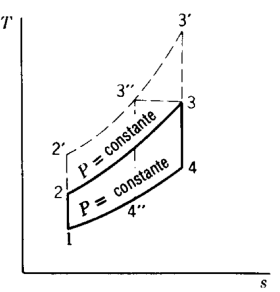
\includegraphics[scale=0.45]{ch9/image12.png}
	\captionof{figure}{ }
		\end{wrapfigure}			
	Analysons le rendement. On se rend compte que quand $\Pi$ augmente (avec $T_3/T_2$ constant), 
	le rendement fait de même : le cycle devient $1-2'-3'-4-1$. Ceci implique que $w'>w, |q_L'|=|q_L|$.\\
	En pratique, la température $T_3$ est limitée de sorte que lorsque $\Pi$ augmente avec 
	$T_3$ constante, le cycle devient $1-2'-3"-4"-1$. Calculons dès lors l'expression du 
	travail pour un tel cycle :
	\begin{equation}
	w = (h_3-h_4)-(h_2-h_1) = c_p(T_3-T_4)-c_p(T_2-T_1)
	\end{equation}
	En mettant $T_1$ en évidence, on peut obtenir
	\begin{equation}
	w = c_pT_1\left[\left(\dfrac{T_3}{T_1}-\dfrac{T_4}{T_1}\right)-\left(\dfrac{T_2}{T_1}-1\right)
	\right] = 
	c_pT_1\left[\dfrac{T_3}{T_1}\left(1-\dfrac{T_4}{T_3}\right)-\left(\dfrac{T_2}{T_1}-1\right)
	\right]
	\end{equation}
					\begin{wrapfigure}[10]{r}{6.5cm}
					\vspace{-5mm}
	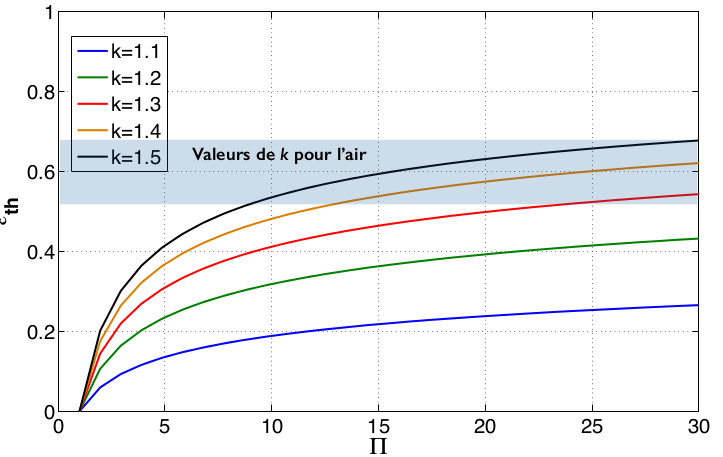
\includegraphics[scale=0.3]{ch9/image13.png}
	\captionof{figure}{ }
		\end{wrapfigure}
	On obtient finalement
	\begin{equation}
	w = c_p.T_1\left[\dfrac{T_3}{T_1}\left(1-\dfrac{1}{\Pi^{\frac{k-1}{k}}}\right)-\left(
	\Pi^{\frac{k-1}{k}}-1\right)\right]
	\end{equation}

	En dérivant cette expression par rapport à $\Pi^\lambda$, il est possible de trouver le 
	travail maximum\footnote{On pose $\lambda = \frac{k-1}{k}$.} :
	\begin{equation}
	\dfrac{dw}{d\Pi^\lambda} = 0 \Leftrightarrow \Pi^{2\lambda} = \dfrac{T_3}{T_1}
	\end{equation}
	En en tire 
	\begin{equation}
	\Pi = \left(\dfrac{T_3}{T_1}\right)^{\frac{1}{2\lambda}} = \left(\dfrac{T_3}{T_1}\right)^{
	\frac{k}{2(k-1)}}
	\end{equation}
	Le rendement peut alors s'écrire 
	\begin{equation}
	\epsilon_{th} = 1-\sqrt{\dfrac{T_1}{T_3}}
	\end{equation}
	
		\subsubsection{Cycle réel}
							\begin{wrapfigure}[11]{l}{4.5cm}
					\vspace{-5mm}
	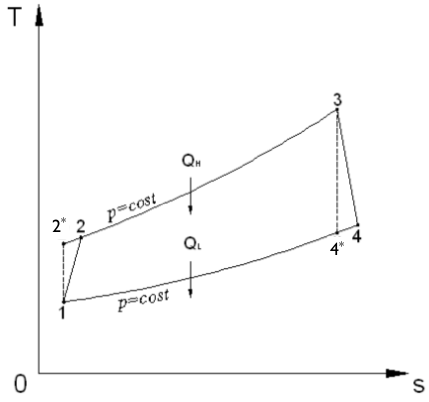
\includegraphics[scale=0.3]{ch9/image14.png}
	\captionof{figure}{ }
		\end{wrapfigure}
		Nous avons jusqu'ici discuter du cas idéal mais il est clair que pour obtenir une 
		description réelle il faut introduire les différentes pertes. Commençons par les 
		pertes par dissipation visqueuses (rendements isentropiques). Nous pouvons simplifier 
		les $c_p$ pour obtenir
		\begin{equation}
		\eta_c = \dfrac{h_{2*}-h_1}{h_2-h_1}=\dfrac{T_{2*}-T_1}{T_2-T_1} \;
		\eta_t = \dfrac{h_3-h_4}{h_3-h_{4*}} =\dfrac{T_3-T_4}{T_3-T_{4*}}
		\end{equation}
		Il faut également tenir compte des pertes de charges et des pertes mécaniques. Sur 
		le diagramme ci-contre, on peut symboliser ceci par les lignes 1-2 et 3-4 qui ne 
		représentent \textbf{pas} une transformation mais jusque les états finaux\footnote{On 
		ne peut pas représenter ici une transformation réversible}.\\
		
		L'efficacité du cycle réel est alors modifiée par la présence des rendements isentropiques. 
		Nous avions
		\begin{equation}
		\epsilon_{th} = \dfrac{w_{net}}{q_{in}} = \dfrac{c_p(T_3-T_4)-c_p(T_2-T_1)}{c_p(T_3-T_2)}
		\end{equation}
		En introduisant les expressions, on peut obtenir (calculs non détaillés ici, mais l'idée 
		est d'ajouter et soustraire $T_1$ au numérateur pour faire apparaître $T_{2*}-T_1$ et 
		l'exprimer avec le rendement isentropique du compresseur) :
		\begin{equation}
		\epsilon_{th} = \dfrac{\tau\eta_t\left(1-\dfrac{1}{\Pi^\lambda}\right)-\dfrac{\left(
		\Pi^\lambda-1\right)}{\eta_c}}{(\tau-1)-\dfrac{(\Pi^\lambda-1)}{\eta_c}}
		\end{equation}
		où $\tau = T_3/T_1$. On remarque que \\
		
		\retenir{L'efficacité du cycle réel est fonction de la température maximale du cycle 
		$T_3$ ainsi que des rendements isentropiques $\eta_c$ et $\eta_t$.}\
		
		Les graphiques de l'efficacité sont aussi modifiés : ce n'est plus du tout 
		asymptotique, on tend ici vers un maximum avant de décroître.
		\begin{center}
		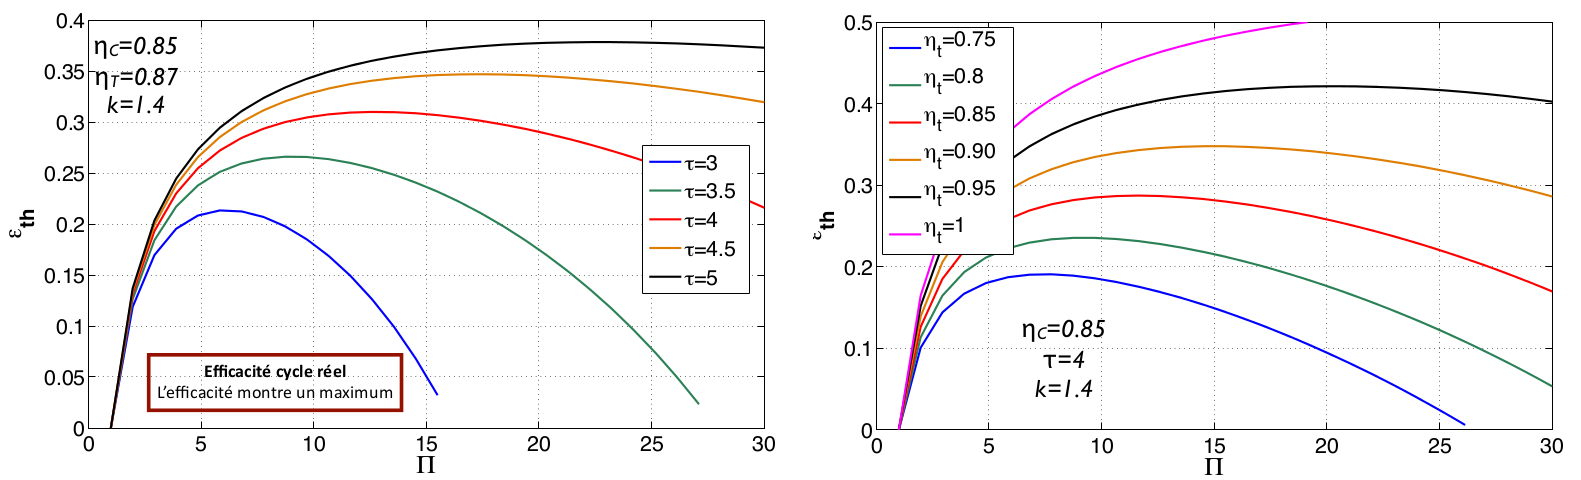
\includegraphics[scale=0.3]{ch9/image15.png}
		\captionof{figure}{ }
		\end{center}
		Si on fixe les $\eta_c/\eta_t, k$ on observe le diagramme de gauche représentant 
		l'efficacité $\epsilon = f(\Pi,\tau)$. Si on fait cette fois-ci varier $\eta_t$ 
		pour obtenir le graphe $\epsilon = f(\Pi,\eta_t)$ (droite) on voit que l'effet d'une 
		variation est \textsc{énorme} : avoir une turbine plus ou moins isentropique 
		joue énormément.
		
		
		\subsubsection{Cycle à récupération}
		L'avantage de chauffer l'air est que l'on doit moins utiliser nos échangeurs 
		thermiques : on gagne donc en chaleur. 
		\begin{center}
		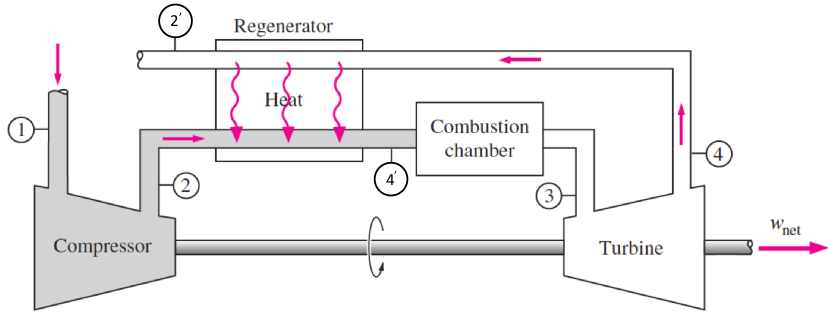
\includegraphics[scale=0.3]{ch9/image16.png}
		\captionof{figure}{ }
		\end{center}	
		Dans le meilleur des cas, $T_2'=T_2$ et $T_4'=T_4$ mais ne rêvons pas car cela 
		signifierait un $\Delta T=0$. Calculons l'efficacité du cycle de Joule à 
		récupération :
		\begin{equation}
		\epsilon_{th} = \dfrac{c_p(T_3-T_4)-c_p(T_2-T_1)}{c_p(T_3-T_2)} = 1-\dfrac{T_2-T_1}{
		T_3-T_4} = 1-\dfrac{T_1}{T_3}\dfrac{\left(\dfrac{T_2}{T_1}-1\right)}{\left(1-
		\dfrac{T_4}{T_3}\right)}
		\end{equation}
		En ré-écrivant ceci à l'aide de $\Pi^{\frac{k-1}{k}}$ on obtient
		\begin{equation}
		\epsilon_{th} = 1-\dfrac{T_1}{T_3}\dfrac{\left(\Pi^{\frac{k-1}{k}}-1 \right)}{\left( 
		1-\dfrac{1}{\Pi^{\frac{k-1}{k}}}\right)} = 1-\dfrac{T_1}{T_3}\Pi^{\frac{k-1}{k}}
		\end{equation}
		Et finalement : 
		
		\retenir{\begin{equation}
		\epsilon_{th} = 1-\dfrac{\Pi^{\frac{k-1}{k}}}{\tau} > \epsilon_{JB}
		\end{equation}
		Cette efficacité augmente avec $\tau$ (plus de chaleur disponible pour la 
		récupération) et diminue avec $\Pi$ (moins de chaleur disponible pour la 
		récupération)}\ 
		
		Au niveau des diagramme, quelle est la différence ? Avant nous avions $h_3-h_2$ 
		et maintenant on considère $h_4'$, la partie 2-4' n'a plus de transfert de 
		chaleur et l'effet onéreux n'est plus que $h_3-h_4"$. Le principal avantage 
		c'est qu'on récupère plus de chaleur. Par contre, il a fallu mettre un tuyau 
		en plus et la construction est devenue plus cher (bien qu'énergétiquement plus 
		avantageux).

		\begin{center}
		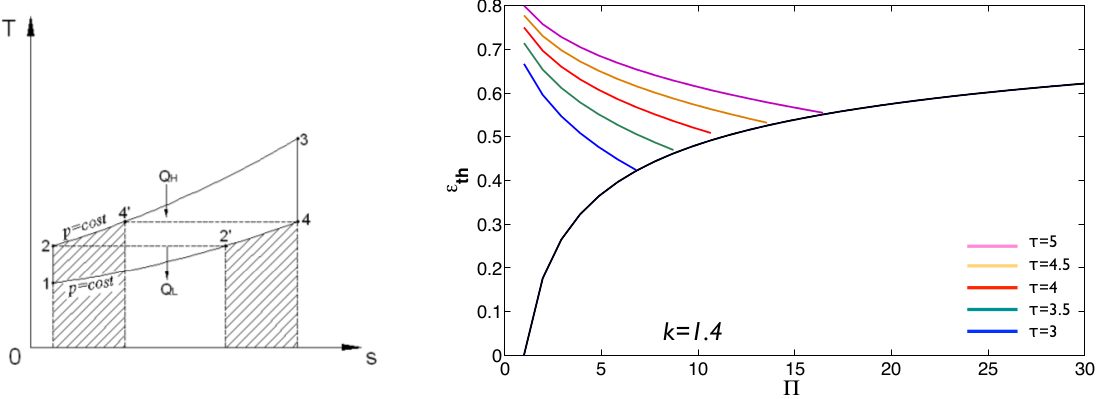
\includegraphics[scale=0.35]{ch9/image17.png}
		\captionof{figure}{Cycle à récupération idéal}
		\end{center}			
		
		Un tel cycle n'est pas toujours possible, il faut que la température à la  sortie 
		de la turbine soit plus élevée qu'à l'entrée du compresseur. Graphiquement, si 
		$T_4<T_2$ nous somme au delà de la courbe noire ci-dessus, représentant 
		l'efficacité de Joule idéale. Si ce n'est pas le cas, il faut considérer les 
		différentes courbes en fonction de $\tau$ à gauche de cette courbe. Notons que 
		l'intersection de ces courbes correspond à $T_4=T_2$.\footnote{Tout ceci est pour 
		le cas idéal. Pour le cas réel, voir slides 50-52. L'efficacité réelle est définie 
		par rapport au seuil enthalpique maximum que l'on pourrait obtenir (4-2)}
		
	
		\subsubsection{Cycle à	compression	et détente	étagée}
		Le but est toujours de maximiser le travail dans la turbine. Pour avoir du travail 
		dans la turbine (travail isotherme > travail adiabatique), il faut "payer" un travail 
		au compresseur : il faut donc minimiser ce travail. Une autre façon de voir les choses 
		est de penser au diagramme $p-V$. Nous sommes en système ouvert $w = \int vdp$. Le travail 
		d'une adiabatique (pour la compression) ($k=1.4$)	 projeté sur l'axe $P$ sera plus 
		important que le travail d'une isotherme ($k=1$). Cependant, pour passer au point 1 au 
		point 2 (détente) on souhaite avoir un travail maximal : c'est l'isotherme qui donne 
		un travail maximal dans cette situation\footnote{Pour s'en rendre compte, tracer un 
		diagramme !}
		
				\begin{center}
		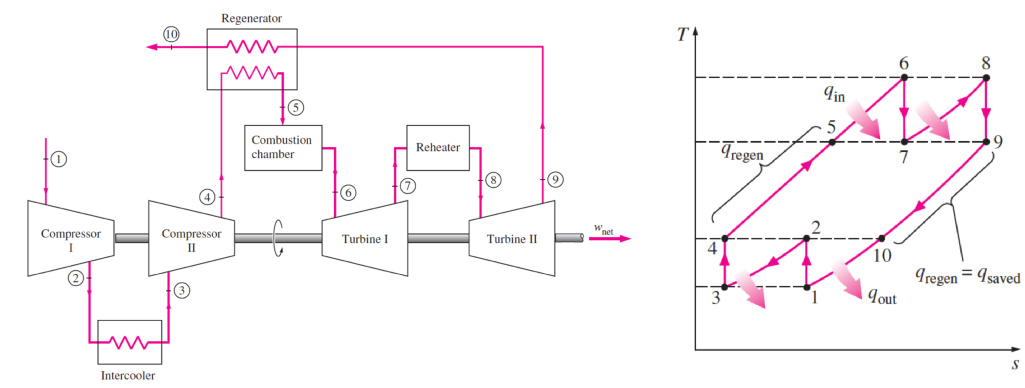
\includegraphics[scale=0.4]{ch9/image18.png}
		\captionof{figure}{Cycle à compression et détente étagée}
		\end{center}			
		
		L'installation fonctionne de la sorte : après une première compression, la température 
		est refroidie puis le gaz est à nouveau compressé. Le coût de l'installation augmente 
		mais c'est bien mieux énergétiquement. A la sortie de la turbine (7) réchauffer le gaz
		avant d'entrer dans la seconde turbine est aussi plus avantageux. Le souci d'une telle 
		installation est qu'il faut tout avoir en double.\\
		Le cycle du turboréacteur repose sur une variante du cycle de Joule.
		
	\subsection{Cycle de Ericsson}
	
	
	
	
	
	
	
	
	
	
	
